
\subsection{N-band imaging recipes}
\label{ssec:recipes_img_n}
%------------------------------------------------------------------------------------------------------------------
\subsubsection{\REC*{metis_n_img_flat}:  Flatfielding}
\label{n_img_flatfield}
\label{rec:n_img_flatfield}
\label{sssec:n_img_flatfield}
\label{n_img_flat}
\label{rec:n_img_flat}
\label{sssec:n_img_flat}
\label{metis_n_img_flat}
\label{rec:metis_n_img_flat}
\label{sssec:metis_n_img_flat}

The purpose of the flat-field calibration is to determine
pixel-to-pixel gain variations and large scale illumination variations
(due to inhomogeneities of optical elements in the telescope or
instrument). Calibration frames are obtained either during day time
using the black-body lamp of the \ac{WCU} (internal flats) or by taken
images of the twilight sky (twilight flats). Advantages and
disadvantages of the two types of flat are discussed in
\cite{METIS-calibration_plan}.

MIR detectors are typically unstable in that they show gain
fluctuations on rather short time scales, hence science exposures may
have a different flat-field structure from those captured by the
calibration flats.  The GeoSnap detector is more linear
than the H2RG detectors, but should be flat-fielded anyway.
N-band flat fields will also be taken for quality control and monitoring purposes.

Since the operational concept for twilight flats needs to be refined
during commissioning at the telescope, the current recipe design is
primarily valid for internal flats.

This recipe creates a master flat for the GeoSnap detector (N-band
imaging) from lamp or sky images matched by various setup parameters
as detailed below.  A set of internal flats includes a number of
exposures with \CODE{LAMP OFF}, which will be used for dark
subtraction. For twilight flats a master dark will be subtracted. The
master flat is obtained by the slope of a linear fit of the pixel
values against the illumination level of the exposures.

The quality control parameters give various statistics for each input
frame (mean, standard deviation, etc.), the standard deviation of the
normalised master flat and the number of bad pixels identified by the
recipe. If a bad-pixel map is provided on input, it is updated,
otherwise a new one is created.

\begin{recipedef}
  Name:                & \REC{metis_n_img_flat} \\
  Purpose:             & Create master flat for N band detectors \\
%  Requirements:        & \REQ{METIS-XXXX} \\
%  Type:                & Calibration | Science | Technical \\
%  Templates:           & \TPL{...} \\
  Primary input:       & \RAW{N_FLAT_LAMP_RAW} or \RAW{N_FLAT_TWILIGHT_RAW} (N$\times$) \\
  Secondary inputs:    & \PROD{BADPIX_MAP_GEO} (optional) \\
                       & \hyperref[dataitem:gain_map_det]{\STATCALIB*{GAIN_MAP_GEO}} \\
                       & \hyperref[dataitem:linearity_det]{\PROD*{LINEARITY_GEO}} \\
                       & \PROD{MASTER_DARK_GEO} \\
                       & \EXTCALIB{PERSISTENCE_MAP} (optional) \\
  Matched keywords:    & \FITS{DET.DIT} \\
                       & \FITS{DET.NDIT} \\
                       & \FITS{DRS.FILTER} \\
  Parameters:          & \CODE{metis_n_img_flat.stacking.method}: string\newline Name of the method used to combine the input images (\texttt{add}, \underline{\texttt{average}}, \texttt{median}) \\
                       & \CODE{metis_n_img_flat.outliers.kappa_low}: float\newline Lower threshold for bad pixels, default \texttt{10.0} \\
                       & \CODE{metis_n_img_flat.outliers.kappa_high}: float\newline Upper threshold for bad pixels, default \texttt{10.0} \\
  Algorithm:           & For internal flats: call \REC{metis_det_dark} with LAMP OFF im ages to create dark frame. \\
                       & Subtract internal dark or master dark from flat exposures. \\
                       & Call \REC{metis_n_img_flat} to fit slope of pixel values against illumination level. \\
                       & Frames with the same exposure time will be averaged. \\
                       & Compute median or average of input frames to improve statistics. \\
                       & Call metis\_update\_n\_flat\_mask to flag deviant pixels. \\
  Output data:         & \PROD{BADPIX_MAP_GEO} \\
                       & \PROD{MASTER_IMG_FLAT_LAMP_N} or \PROD{MASTER_IMG_FLAT_TWILIGHT_N} \\
%  Expected accuracies: & \\
  QC1 parameters:      & \QC{QC N FLAT MEAN} \\
                       & \QC{QC N FLAT MEDIAN MAX} \\
                       & \QC{QC N FLAT MEDIAN MIN} \\
                       & \QC{QC N FLAT MEDIAN RMS} \\
                       & \QC{QC N FLAT RMS} \\
                       & \QC{QC N MFLAT NBADPIX} \\
                       & \QC{QC N MFLAT RMS} \\
\end{recipedef}



\begin{figure}[hb]
  \centering
    \def \globalscale {0.700000}
    \fontsize{10}{12}\selectfont
    %% Flowchart of metis_n_img_flat, generated by metisp/drld/generate_drld.py -- do not edit

% ADDING NEW DEFINITIONS -------------------------------------------- start
\definecolor{listingbg}{gray}{0.95}
\definecolor{darkgreen}{rgb}{0.0, 0.7, 0.0}
\definecolor{darkblue} {rgb}{0.0, 0.0, 0.7}
\definecolor{cyan} {rgb}{0.0, 0.4, 0.4}
\definecolor{darkred}  {rgb}{0.7, 0.0, 0.0}
\definecolor{darkorange}{rgb}{1.0, 0.49, 0.0}
\definecolor{violet}{rgb}{255, 0, 255}
\definecolor{turq}{rgb}{0.0, 0.7, 0.8}
\definecolor{fits}{rgb}{0.4, 0.1, 1}


\makeatletter
\lstdefinestyle{RAWstyle}{%
  basicstyle=\ttfamily\color{black}%
  \lst@ifdisplaystyle\scriptsize\fi}

\lstdefinestyle{PARstyle}{%
  basicstyle=\ttfamily\color{black}%
  \lst@ifdisplaystyle\scriptsize\fi}

\lstdefinestyle{DRLstyle}{%
  basicstyle=\ttfamily\color{black}%
  \lst@ifdisplaystyle\scriptsize\fi}

\lstdefinestyle{RECstyle}{%
  basicstyle=\ttfamily\color{black}%
  \lst@ifdisplaystyle\scriptsize\fi}

\lstdefinestyle{QCstyle}{%
  basicstyle=\ttfamily\color{black}%
  \lst@ifdisplaystyle\scriptsize\fi}

\lstdefinestyle{TPLstyle}{%
  basicstyle=\ttfamily\color{black}%
  \lst@ifdisplaystyle\scriptsize\fi}

\lstdefinestyle{PRODstyle}{%
  basicstyle=\ttfamily\color{black}%
  \lst@ifdisplaystyle\scriptsize\fi}

\lstdefinestyle{EXTCALIBstyle}{%
  basicstyle=\ttfamily\color{black}%
  \lst@ifdisplaystyle\scriptsize\fi}

\lstdefinestyle{STATCALIBstyle}{%
  basicstyle=\ttfamily\color{black}%
  \lst@ifdisplaystyle\scriptsize\fi}

\lstdefinestyle{FITSstyle}{%
  basicstyle=\ttfamily\color{black}%
  \lst@ifdisplaystyle\scriptsize\fi}
\makeatother

\input{recipe_config}
%% The picture is set in a box and only scaled down when it would not fit the page.
\ifdefined\flowchartbox\else\newsavebox{\flowchartbox}\fi
\sbox{\flowchartbox}{%
\begin{tikzpicture}
  [x=1cm,
  y=-1cm,
  align=center,
  node distance=2cm and 3.5cm,
  redstep/.append style={minimum height=0.8cm, text width=3.8cm}]
  \sffamily
  \pic (start){start};
  \node (input) [below=0.75cm of start-m, input] {%
    \textsl{N} \RAW{N_FLAT_LAMP_RAW} \\[-0.5ex] {\footnotesize or} \\[-0.5ex] \textsl{N} \RAW{N_FLAT_TWILIGHT_RAW}};

  %% algorithm steps
  \node (step_detectorsignatureremoval) [below=5.6cm of input, redstep]{%
    detector signature removal};
  \node (step_linearfitslope) [below=0.6cm of step_detectorsignatureremoval, redstep]{%
    linear fit (slope)};
  \pic (stop) [below=3.16cm of step_linearfitslope] {stop};

  \draw [connection_arrow] (start-m) -- (input);
  \draw [connection_arrow] (input) -- (step_detectorsignatureremoval);
  \draw [connection_arrow] (step_detectorsignatureremoval) -- (step_linearfitslope);
  \draw [connection_arrow] (step_linearfitslope) -- (stop-t);

  %% calibration inputs, attached above the step that consumes them
  \node (connect_badpixmap) [connection] at ($(input.south) + (0, 0.97)$) {};
  \node (badpixmap) [left=of connect_badpixmap, calproduct] {\PROD{BADPIX_MAP_GEO}};
  \draw [connection_arrow, dashed] (badpixmap) -- (connect_badpixmap);
  \node (connect_gainmap) [connection] at ($(input.south) + (0, 1.98)$) {};
  \node (gainmap) [left=of connect_gainmap, external] {\hyperref[dataitem:gain_map_det]{\STATCALIB*{GAIN_MAP_GEO}}};
  \draw [connection_arrow] (gainmap) -- (connect_gainmap);
  \node (connect_linearity) [connection] at ($(input.south) + (0, 2.98)$) {};
  \node (linearity) [left=of connect_linearity, calproduct] {\hyperref[dataitem:linearity_det]{\PROD*{LINEARITY_GEO}}};
  \draw [connection_arrow] (linearity) -- (connect_linearity);
  \node (connect_masterdark) [connection] at ($(input.south) + (0, 3.98)$) {};
  \node (masterdark) [left=of connect_masterdark, calproduct] {\PROD{MASTER_DARK_GEO}};
  \draw [connection_arrow] (masterdark) -- (connect_masterdark);
  \node (connect_persistencemap) [connection] at ($(input.south) + (0, 4.97)$) {};
  \node (persistencemap) [left=of connect_persistencemap, external] {\EXTCALIB{PERSISTENCE_MAP}};
  \draw [connection_arrow, dashed] (persistencemap) -- (connect_persistencemap);

  %% products, attached below the step that produces them
  \node (connect_badpixmap) [connection] at ($(step_linearfitslope.south) + (0, 0.62)$) {};
  \node (badpixmap) [right=of connect_badpixmap, calproduct] {\PROD{BADPIX_MAP_GEO}};
  \draw [connection_arrow] (connect_badpixmap) -- (badpixmap);
  \node (connect_masterflat) [connection] at ($(step_linearfitslope.south) + (0, 1.98)$) {};
  \node (masterflat) [right=of connect_masterflat, calproduct] {\PROD{MASTER_IMG_FLAT_LAMP_N} \\[-0.5ex] {\footnotesize or} \\[-0.5ex] \PROD{MASTER_IMG_FLAT_TWILIGHT_N}};
  \draw [connection_arrow] (connect_masterflat) -- (masterflat);

  \draw [frame] ($(input.south) + (-2.85, 0.12)$) rectangle
  ($(step_linearfitslope.south) + (2.85, 2.7600000000000002)$);
  \node [framecolor, anchor=north west] at ($(input.south) + (-2.85, 0.12)$) {%
    \REC{metis_n_img_flat}};
\end{tikzpicture}}%
\ifdim\ht\flowchartbox>\dimexpr\textheight-4\baselineskip\relax
  \resizebox{!}{\dimexpr\textheight-4\baselineskip\relax}{\usebox{\flowchartbox}}%
\else\ifdim\wd\flowchartbox>\linewidth
  \resizebox{\linewidth}{!}{\usebox{\flowchartbox}}%
\else
  \usebox{\flowchartbox}%
\fi\fi

% ADDING NEW DEFINITIONS -------------------------------------------- start
\definecolor{listingbg}{gray}{0.95}
\definecolor{darkgreen}{rgb}{0.0, 0.7, 0.0}
\definecolor{darkblue} {rgb}{0.0, 0.0, 0.7}
\definecolor{cyan} {rgb}{0.0, 0.4, 0.4}
\definecolor{darkred}  {rgb}{0.7, 0.0, 0.0}
\definecolor{darkorange}{rgb}{1.0, 0.49, 0.0}
\definecolor{violet}{rgb}{255, 0, 255}
\definecolor{turq}{rgb}{0.0, 0.7, 0.8}
\definecolor{fits}{rgb}{0.4, 0.1, 1}


\makeatletter
\lstdefinestyle{RAWstyle}{%
  basicstyle=\ttfamily\color{fits}%
  \lst@ifdisplaystyle\scriptsize\fi}

\lstdefinestyle{PARstyle}{%
  basicstyle=\ttfamily\color{cyan}%
  \lst@ifdisplaystyle\scriptsize\fi}

\lstdefinestyle{DRLstyle}{%
  basicstyle=\ttfamily\color{violet}%
  \lst@ifdisplaystyle\scriptsize\fi}

\lstdefinestyle{RECstyle}{%
  basicstyle=\ttfamily\color{darkgreen}%
  \lst@ifdisplaystyle\scriptsize\fi}

%% Write QC parameters like this: \QC{QC_SOMETHING_OR_OTHER}
\lstdefinestyle{QCstyle}{%
  basicstyle=\ttfamily\color{darkblue}%
  \lst@ifdisplaystyle\scriptsize\fi}

%% Write templates like this: \TPL{DARK_LM}
\lstdefinestyle{TPLstyle}{%
  basicstyle=\ttfamily\color{darkred}%
  \lst@ifdisplaystyle\scriptsize\fi}

%% Write products like this: \PROD{SOME_THING}
\lstdefinestyle{PRODstyle}{%
  basicstyle=\ttfamily\color{darkorange}%
  \lst@ifdisplaystyle\scriptsize\fi}

%% external calib files
\lstdefinestyle{EXTCALIBstyle}{%
  basicstyle=\ttfamily\color{Turquoise}%
  \lst@ifdisplaystyle\scriptsize\fi}

% static calib files
\lstdefinestyle{STATCALIBstyle}{%
  basicstyle=\ttfamily\color{teal}%
  \lst@ifdisplaystyle\scriptsize\fi}

% static calib files
\lstdefinestyle{FITSstyle}{%
  basicstyle=\ttfamily\color{black}%
  \lst@ifdisplaystyle\scriptsize\fi}
\makeatother


  \caption[Recipe: \REC*{metis_n_img_flat}]{\REC*{metis_n_img_flat} --
    creation of \CODE{IMG_N} master flatfield}
  \label{fig:metis_n_img_flat}
\end{figure}

%%%%%%%
%------------------------------------------------------------------------------------------------------------------
\subsubsection{\REC*{metis_n_img_chopnod}:  Chop-nod combination}
\label{img_n_chopnod}
\label{rec:img_n_chopnod}
\label{rec:metis_n_img_chopnod}
\label{sssec:img_n_chopnod}

This recipe combines a set of exposures taken at all positions of a
defined chop-nod pattern and adds/subtracts them into a single
chop/nod difference image. Depending on the actual chop-nod pattern,
this image will contain one or more positive and negative beams.
See Section~\ref{sssec:nbandsbackgroundsubtracion} for more information
on the background subtraction.

The GeoSnap detectors will have a substantial number of bad pixels.
The N-band observations therefore require extensive dithering to mitigated bad pixels.
The master flat will have to be divided into the chop half-cycle images before the dither correction is applied.

% https://polarion.astron.nl/polarion/#/project/METIS/workitem?id=METIS-3091
This recipe analyses the masked detector regions for channel offset correction, crosstalk (see Section~\ref{ssec:criticaldetetctormasks}) and removal of detector artefacts (electronic ghosts).
The edges of the N-band detector will be behind a cold mask on all four sides.
%The width of the mask will be at least 26 pixels and no larger than 32 pixels.


\begin{recipedef}
  Name:                & \REC{metis_n_img_chopnod} \\
  Purpose:             & Basic science image data processing \\
%  Requirements:        & \REQ{METIS-XXXX} \\
%  Type:                & Calibration | Science | Technical \\
%  Templates:           & \TPL{...} \\
  Primary input:       & \RAW{N_IMAGE_SCI_RAW} or \RAW{N_IMAGE_STD_RAW} (1--N) \\
  Secondary inputs:    & \PROD{BADPIX_MAP_GEO} (optional) \\
                       & \hyperref[dataitem:gain_map_det]{\STATCALIB*{GAIN_MAP_GEO}} \\
                       & \hyperref[dataitem:linearity_det]{\PROD*{LINEARITY_GEO}} \\
                       & \PROD{MASTER_DARK_GEO} \\
                       & \PROD{MASTER_IMG_FLAT_LAMP_N} or \PROD{MASTER_IMG_FLAT_TWILIGHT_N} \\
                       & \EXTCALIB{PERSISTENCE_MAP} (optional) \\
  Matched keywords:    & \FITS{DET.DIT} \\
                       & \FITS{DET.NDIT} \\
                       & \FITS{DRS.FILTER} \\
  Parameters:          & \CODE{metis_n_img_chopnod.stacking.method}\newline Name of the method used to combine the input images (\texttt{add}, \texttt{average}, \texttt{median}), default \texttt{add} \\
  Algorithm:           & Remove crosstalk, correct non-linearity \\
                       & Analyse and optionally remove masked regions \\
                       & Subtract dark, divide by flat \\
                       & Remove blank sky pattern \\
  Output data:         & \PROD{N_SCI_BKG_SUBTRACTED} or \PROD{N_STD_BKG_SUBTRACTED} \\
%  Expected accuracies: & \\
  QC1 parameters:      & \QC{QC N IMG PEAK CNTS} \\
\end{recipedef}



\newgeometry{bottom=0.5cm, right=0.5cm, left=0.5cm}
 \begin{figure}[hb]
  \centering
  \def \globalscale {0.700000}
  \fontsize{10}{12}\selectfont
  %% Flowchart of metis_n_img_chopnod, generated by metisp/drld/generate_drld.py -- do not edit

% ADDING NEW DEFINITIONS -------------------------------------------- start
\definecolor{listingbg}{gray}{0.95}
\definecolor{darkgreen}{rgb}{0.0, 0.7, 0.0}
\definecolor{darkblue} {rgb}{0.0, 0.0, 0.7}
\definecolor{cyan} {rgb}{0.0, 0.4, 0.4}
\definecolor{darkred}  {rgb}{0.7, 0.0, 0.0}
\definecolor{darkorange}{rgb}{1.0, 0.49, 0.0}
\definecolor{violet}{rgb}{255, 0, 255}
\definecolor{turq}{rgb}{0.0, 0.7, 0.8}
\definecolor{fits}{rgb}{0.4, 0.1, 1}


\makeatletter
\lstdefinestyle{RAWstyle}{%
  basicstyle=\ttfamily\color{black}%
  \lst@ifdisplaystyle\scriptsize\fi}

\lstdefinestyle{PARstyle}{%
  basicstyle=\ttfamily\color{black}%
  \lst@ifdisplaystyle\scriptsize\fi}

\lstdefinestyle{DRLstyle}{%
  basicstyle=\ttfamily\color{black}%
  \lst@ifdisplaystyle\scriptsize\fi}

\lstdefinestyle{RECstyle}{%
  basicstyle=\ttfamily\color{black}%
  \lst@ifdisplaystyle\scriptsize\fi}

\lstdefinestyle{QCstyle}{%
  basicstyle=\ttfamily\color{black}%
  \lst@ifdisplaystyle\scriptsize\fi}

\lstdefinestyle{TPLstyle}{%
  basicstyle=\ttfamily\color{black}%
  \lst@ifdisplaystyle\scriptsize\fi}

\lstdefinestyle{PRODstyle}{%
  basicstyle=\ttfamily\color{black}%
  \lst@ifdisplaystyle\scriptsize\fi}

\lstdefinestyle{EXTCALIBstyle}{%
  basicstyle=\ttfamily\color{black}%
  \lst@ifdisplaystyle\scriptsize\fi}

\lstdefinestyle{STATCALIBstyle}{%
  basicstyle=\ttfamily\color{black}%
  \lst@ifdisplaystyle\scriptsize\fi}

\lstdefinestyle{FITSstyle}{%
  basicstyle=\ttfamily\color{black}%
  \lst@ifdisplaystyle\scriptsize\fi}
\makeatother

\input{recipe_config}
%% The picture is set in a box and only scaled down when it would not fit the page.
\ifdefined\flowchartbox\else\newsavebox{\flowchartbox}\fi
\sbox{\flowchartbox}{%
\begin{tikzpicture}
  [x=1cm,
  y=-1cm,
  align=center,
  node distance=2cm and 3.5cm,
  redstep/.append style={minimum height=0.8cm, text width=3.8cm}]
  \sffamily
  \pic (start){start};
  \node (input) [below=0.75cm of start-m, input] {%
    \textsl{N} \RAW{N_IMAGE_SCI_RAW} \\[-0.5ex] {\footnotesize or} \\[-0.5ex] \textsl{N} \RAW{N_IMAGE_STD_RAW}};

  %% algorithm steps
  \node (step_correctnonlinearity) [below=3.6cm of input, redstep]{%
    Correct non-linearity};
  \node (step_correctpersistence) [below=1.25cm of step_correctnonlinearity, redstep]{%
    Correct persistence};
  \node (step_subtractdark) [below=1.25cm of step_correctpersistence, redstep]{%
    subtract dark};
  \node (step_dividebyflat) [below=1.96cm of step_subtractdark, redstep]{%
    divide by flat};
  \node (step_analyseandremovemaskedre) [below=0.6cm of step_dividebyflat, redstep]{%
    analyse and remove masked regions};
  \pic (stop) [below=2.16cm of step_analyseandremovemaskedre] {stop};

  \draw [connection_arrow] (start-m) -- (input);
  \draw [connection_arrow] (input) -- (step_correctnonlinearity);
  \draw [connection_arrow] (step_correctnonlinearity) -- (step_correctpersistence);
  \draw [connection_arrow] (step_correctpersistence) -- (step_subtractdark);
  \draw [connection_arrow] (step_subtractdark) -- (step_dividebyflat);
  \draw [connection_arrow] (step_dividebyflat) -- (step_analyseandremovemaskedre);
  \draw [connection_arrow] (step_analyseandremovemaskedre) -- (stop-t);

  %% calibration inputs, attached above the step that consumes them
  \node (connect_badpixmap) [connection] at ($(input.south) + (0, 0.97)$) {};
  \node (badpixmap) [left=of connect_badpixmap, calproduct] {\PROD{BADPIX_MAP_GEO}};
  \draw [connection_arrow, dashed] (badpixmap) -- (connect_badpixmap);
  \node (connect_gainmap) [connection] at ($(input.south) + (0, 1.98)$) {};
  \node (gainmap) [left=of connect_gainmap, external] {\hyperref[dataitem:gain_map_det]{\STATCALIB*{GAIN_MAP_GEO}}};
  \draw [connection_arrow] (gainmap) -- (connect_gainmap);
  \node (connect_linearity) [connection] at ($(input.south) + (0, 2.98)$) {};
  \node (linearity) [left=of connect_linearity, calproduct] {\hyperref[dataitem:linearity_det]{\PROD*{LINEARITY_GEO}}};
  \draw [connection_arrow] (linearity) -- (connect_linearity);
  \node (connect_persistencemap) [connection] at ($(step_correctnonlinearity.south) + (0, 0.62)$) {};
  \node (persistencemap) [left=of connect_persistencemap, external] {\EXTCALIB{PERSISTENCE_MAP}};
  \draw [connection_arrow, dashed] (persistencemap) -- (connect_persistencemap);
  \node (connect_masterdark) [connection] at ($(step_correctpersistence.south) + (0, 0.62)$) {};
  \node (masterdark) [left=of connect_masterdark, calproduct] {\PROD{MASTER_DARK_GEO}};
  \draw [connection_arrow] (masterdark) -- (connect_masterdark);
  \node (connect_masterflat) [connection] at ($(step_subtractdark.south) + (0, 0.98)$) {};
  \node (masterflat) [left=of connect_masterflat, calproduct] {\PROD{MASTER_IMG_FLAT_LAMP_N} \\[-0.5ex] {\footnotesize or} \\[-0.5ex] \PROD{MASTER_IMG_FLAT_TWILIGHT_N}};
  \draw [connection_arrow] (masterflat) -- (connect_masterflat);

  %% products, attached below the step that produces them
  \node (connect_reduced) [connection] at ($(step_analyseandremovemaskedre.south) + (0, 0.98)$) {};
  \node (reduced) [right=of connect_reduced, sciproduct] {\PROD{N_SCI_BKG_SUBTRACTED} \\[-0.5ex] {\footnotesize or} \\[-0.5ex] \PROD{N_STD_BKG_SUBTRACTED}};
  \draw [connection_arrow] (connect_reduced) -- (reduced);

  \draw [frame] ($(input.south) + (-2.85, 0.12)$) rectangle
  ($(step_analyseandremovemaskedre.south) + (2.85, 1.7600000000000002)$);
  \node [framecolor, anchor=north west] at ($(input.south) + (-2.85, 0.12)$) {%
    \REC{metis_n_img_chopnod}};
\end{tikzpicture}}%
\ifdim\ht\flowchartbox>\dimexpr\textheight-4\baselineskip\relax
  \resizebox{!}{\dimexpr\textheight-4\baselineskip\relax}{\usebox{\flowchartbox}}%
\else\ifdim\wd\flowchartbox>\linewidth
  \resizebox{\linewidth}{!}{\usebox{\flowchartbox}}%
\else
  \usebox{\flowchartbox}%
\fi\fi

% ADDING NEW DEFINITIONS -------------------------------------------- start
\definecolor{listingbg}{gray}{0.95}
\definecolor{darkgreen}{rgb}{0.0, 0.7, 0.0}
\definecolor{darkblue} {rgb}{0.0, 0.0, 0.7}
\definecolor{cyan} {rgb}{0.0, 0.4, 0.4}
\definecolor{darkred}  {rgb}{0.7, 0.0, 0.0}
\definecolor{darkorange}{rgb}{1.0, 0.49, 0.0}
\definecolor{violet}{rgb}{255, 0, 255}
\definecolor{turq}{rgb}{0.0, 0.7, 0.8}
\definecolor{fits}{rgb}{0.4, 0.1, 1}


\makeatletter
\lstdefinestyle{RAWstyle}{%
  basicstyle=\ttfamily\color{fits}%
  \lst@ifdisplaystyle\scriptsize\fi}

\lstdefinestyle{PARstyle}{%
  basicstyle=\ttfamily\color{cyan}%
  \lst@ifdisplaystyle\scriptsize\fi}

\lstdefinestyle{DRLstyle}{%
  basicstyle=\ttfamily\color{violet}%
  \lst@ifdisplaystyle\scriptsize\fi}

\lstdefinestyle{RECstyle}{%
  basicstyle=\ttfamily\color{darkgreen}%
  \lst@ifdisplaystyle\scriptsize\fi}

%% Write QC parameters like this: \QC{QC_SOMETHING_OR_OTHER}
\lstdefinestyle{QCstyle}{%
  basicstyle=\ttfamily\color{darkblue}%
  \lst@ifdisplaystyle\scriptsize\fi}

%% Write templates like this: \TPL{DARK_LM}
\lstdefinestyle{TPLstyle}{%
  basicstyle=\ttfamily\color{darkred}%
  \lst@ifdisplaystyle\scriptsize\fi}

%% Write products like this: \PROD{SOME_THING}
\lstdefinestyle{PRODstyle}{%
  basicstyle=\ttfamily\color{darkorange}%
  \lst@ifdisplaystyle\scriptsize\fi}

%% external calib files
\lstdefinestyle{EXTCALIBstyle}{%
  basicstyle=\ttfamily\color{Turquoise}%
  \lst@ifdisplaystyle\scriptsize\fi}

% static calib files
\lstdefinestyle{STATCALIBstyle}{%
  basicstyle=\ttfamily\color{teal}%
  \lst@ifdisplaystyle\scriptsize\fi}

% static calib files
\lstdefinestyle{FITSstyle}{%
  basicstyle=\ttfamily\color{black}%
  \lst@ifdisplaystyle\scriptsize\fi}
\makeatother


   \caption[Recipe: \REC*{metis_n_img_chopnod}]{\REC*{metis_n_img_chopnod} --
     Combination of chop/nodded images.}
   \label{fig:metis_n_img_chopnod}
 \end{figure}
\restoregeometry

%%%%%%%%%%%%%%%%%%%
\clearpage
\subsubsection{\REC*{metis_n_img_std_process}:  Photometric standard analysis}
\label{n_img_std_process}
\label{rec:n_img_std_process}
\label{ssec:n_img_std_process}
\label{sssec:n_img_std_process}
\label{metis_n_img_std_process}
\label{rec:metis_n_img_std_process}
\label{sssec:metis_n_img_std_process}

This recipe determines the conversion from ADU to physical units from
a chop-nod difference image of a photometric standard star.  The flux
of the standard star is measured in each of the beams of the chop-nod
difference image, averaged and normalised to an exposure time of
1~second. Comparison to the tabulated brightness of the star in the
observing filter yields the conversion factor from
$\mathrm{ADU}\,\mathrm{s}^{-1}$ to
$\mathrm{photons}\,\mathrm{s}^{-1}\,\mathrm{cm}^{-2}$.

QC parameters will include estimates of the sensitivity for the
detection of point sources and surface brightness sensitivity
following~\cite{visir_manual}.

\begin{recipedef}
  Name:                & \REC{metis_n_img_std_process} \\
  Purpose:             & Determine the conversion factor between detector counts and physical source flux \\
%  Requirements:        & \REQ{METIS-XXXX} \\
%  Type:                & Calibration | Science | Technical \\
%  Templates:           & \TPL{...} \\
  Primary input:       & \PROD{N_STD_BKG_SUBTRACTED} (N$\times$) \\
  Secondary inputs:    & \EXTCALIB{FLUXSTD_CATALOG} \\
  Matched keywords:    & \FITS{DRS.FILTER} \\
  Parameters:          & \CODE{metis_n_img_std_process.stacking.method}: string\newline Name of the method used to combine the input images (\texttt{add}, \underline{\texttt{average}}, \texttt{median}, \texttt{sigclip}) \\
  Algorithm:           & Call metis\_n\_calculate\_std\_flux to measure flux in input images \\
                       & call hdrl\_resample\_compute to recenter the images \\
                       & call hdrl\_imagelist\_collapse to stack the images \\
                       & call metis\_n\_calculate\_std\_flux on the stacked image to get flux of the star in detector units \\
                       & call metis\_calculate\_std\_fluxcal to calculate the conversion factor to physical units \\
                       & call metis\_calculate\_detection\_limits to compute background noise (std, rms) and compute detection limits \\
  Output data:         & \PROD{FLUXCAL_TAB} \\
                       & \PROD{N_STD_COMBINED} \\
%  Expected accuracies: & \\
  QC1 parameters:      & \QC{QC N STD AIRMASS} \\
                       & \QC{QC N STD APERTURE CNTS} \\
                       & \QC{QC N AREA SENS} \\
                       & \QC{QC N IMG STD BACKGD RMS} \\
                       & \QC{QC N STD ELLIP} \\
                       & \QC{QC N STD FLUXCONV} \\
                       & \QC{QC N STD FWHM} \\
                       & \QC{QC N STD PEAK CNTS} \\
                       & \QC{QC N SENS} \\
                       & \QC{QC N STD STREHL} \\
\end{recipedef}



\begin{figure}[hb]
    \centering
    \def \globalscale {0.700000}
    \fontsize{10}{12}\selectfont
    %% Flowchart of metis_n_img_std_process, generated by metisp/drld/generate_drld.py -- do not edit

% ADDING NEW DEFINITIONS -------------------------------------------- start
\definecolor{listingbg}{gray}{0.95}
\definecolor{darkgreen}{rgb}{0.0, 0.7, 0.0}
\definecolor{darkblue} {rgb}{0.0, 0.0, 0.7}
\definecolor{cyan} {rgb}{0.0, 0.4, 0.4}
\definecolor{darkred}  {rgb}{0.7, 0.0, 0.0}
\definecolor{darkorange}{rgb}{1.0, 0.49, 0.0}
\definecolor{violet}{rgb}{255, 0, 255}
\definecolor{turq}{rgb}{0.0, 0.7, 0.8}
\definecolor{fits}{rgb}{0.4, 0.1, 1}


\makeatletter
\lstdefinestyle{RAWstyle}{%
  basicstyle=\ttfamily\color{black}%
  \lst@ifdisplaystyle\scriptsize\fi}

\lstdefinestyle{PARstyle}{%
  basicstyle=\ttfamily\color{black}%
  \lst@ifdisplaystyle\scriptsize\fi}

\lstdefinestyle{DRLstyle}{%
  basicstyle=\ttfamily\color{black}%
  \lst@ifdisplaystyle\scriptsize\fi}

\lstdefinestyle{RECstyle}{%
  basicstyle=\ttfamily\color{black}%
  \lst@ifdisplaystyle\scriptsize\fi}

\lstdefinestyle{QCstyle}{%
  basicstyle=\ttfamily\color{black}%
  \lst@ifdisplaystyle\scriptsize\fi}

\lstdefinestyle{TPLstyle}{%
  basicstyle=\ttfamily\color{black}%
  \lst@ifdisplaystyle\scriptsize\fi}

\lstdefinestyle{PRODstyle}{%
  basicstyle=\ttfamily\color{black}%
  \lst@ifdisplaystyle\scriptsize\fi}

\lstdefinestyle{EXTCALIBstyle}{%
  basicstyle=\ttfamily\color{black}%
  \lst@ifdisplaystyle\scriptsize\fi}

\lstdefinestyle{STATCALIBstyle}{%
  basicstyle=\ttfamily\color{black}%
  \lst@ifdisplaystyle\scriptsize\fi}

\lstdefinestyle{FITSstyle}{%
  basicstyle=\ttfamily\color{black}%
  \lst@ifdisplaystyle\scriptsize\fi}
\makeatother

\input{recipe_config}
%% The picture is set in a box and only scaled down when it would not fit the page.
\ifdefined\flowchartbox\else\newsavebox{\flowchartbox}\fi
\sbox{\flowchartbox}{%
\begin{tikzpicture}
  [x=1cm,
  y=-1cm,
  align=center,
  node distance=2cm and 3.5cm,
  redstep/.append style={minimum height=0.8cm, text width=3.8cm}]
  \sffamily
  \pic (start){start};
  \node (input) [below=0.75cm of start-m, input] {%
    N$\times$ \PROD{N_STD_BKG_SUBTRACTED}};

  %% algorithm steps
  \node (step_detectstandardstarinindi) [below=1.6cm of input, redstep]{%
    Detect standard star in individual frames};
  \node (step_shiftandcombineimagesbas) [below=0.6cm of step_detectstandardstarinindi, redstep]{%
    shift and combine images based on the position of the standard star};
  \node (step_measurefluxfromstarinins) [below=1.25cm of step_shiftandcombineimagesbas, redstep]{%
    measure flux from star in instrumental units in combined image};
  \node (step_computeconversionfactort) [below=0.6cm of step_measurefluxfromstarinins, redstep]{%
    compute conversion factor to physical units};
  \node (step_measurebackgroundnoisean) [below=1.25cm of step_computeconversionfactort, redstep]{%
    measure background noise and calculate detection limits};
  \pic (stop) [below=0.9cm of step_measurebackgroundnoisean] {stop};

  \draw [connection_arrow] (start-m) -- (input);
  \draw [connection_arrow] (input) -- (step_detectstandardstarinindi);
  \draw [connection_arrow] (step_detectstandardstarinindi) -- (step_shiftandcombineimagesbas);
  \draw [connection_arrow] (step_shiftandcombineimagesbas) -- (step_measurefluxfromstarinins);
  \draw [connection_arrow] (step_measurefluxfromstarinins) -- (step_computeconversionfactort);
  \draw [connection_arrow] (step_computeconversionfactort) -- (step_measurebackgroundnoisean);
  \draw [connection_arrow] (step_measurebackgroundnoisean) -- (stop-t);

  %% calibration inputs, attached above the step that consumes them
  \node (connect_fluxstdcatalog) [connection] at ($(input.south) + (0, 0.97)$) {};
  \node (fluxstdcatalog) [left=of connect_fluxstdcatalog, external] {\EXTCALIB{FLUXSTD_CATALOG}};
  \draw [connection_arrow] (fluxstdcatalog) -- (connect_fluxstdcatalog);

  %% products, attached below the step that produces them
  \node (connect_imgstdcombined) [connection] at ($(step_shiftandcombineimagesbas.south) + (0, 0.62)$) {};
  \node (imgstdcombined) [right=of connect_imgstdcombined, sciproduct] {\PROD{N_STD_COMBINED}};
  \draw [connection_arrow] (connect_imgstdcombined) -- (imgstdcombined);
  \node (connect_imgfluxcaltable) [connection] at ($(step_computeconversionfactort.south) + (0, 0.62)$) {};
  \node (imgfluxcaltable) [right=of connect_imgfluxcaltable, calproduct] {\PROD{FLUXCAL_TAB}};
  \draw [connection_arrow] (connect_imgfluxcaltable) -- (imgfluxcaltable);

  \draw [frame] ($(input.south) + (-2.85, 0.12)$) rectangle
  ($(step_measurebackgroundnoisean.south) + (2.85, 0.5)$);
  \node [framecolor, anchor=north west] at ($(input.south) + (-2.85, 0.12)$) {%
    \REC{metis_n_img_std_process}};
\end{tikzpicture}}%
\ifdim\ht\flowchartbox>\dimexpr\textheight-4\baselineskip\relax
  \resizebox{!}{\dimexpr\textheight-4\baselineskip\relax}{\usebox{\flowchartbox}}%
\else\ifdim\wd\flowchartbox>\linewidth
  \resizebox{\linewidth}{!}{\usebox{\flowchartbox}}%
\else
  \usebox{\flowchartbox}%
\fi\fi

% ADDING NEW DEFINITIONS -------------------------------------------- start
\definecolor{listingbg}{gray}{0.95}
\definecolor{darkgreen}{rgb}{0.0, 0.7, 0.0}
\definecolor{darkblue} {rgb}{0.0, 0.0, 0.7}
\definecolor{cyan} {rgb}{0.0, 0.4, 0.4}
\definecolor{darkred}  {rgb}{0.7, 0.0, 0.0}
\definecolor{darkorange}{rgb}{1.0, 0.49, 0.0}
\definecolor{violet}{rgb}{255, 0, 255}
\definecolor{turq}{rgb}{0.0, 0.7, 0.8}
\definecolor{fits}{rgb}{0.4, 0.1, 1}


\makeatletter
\lstdefinestyle{RAWstyle}{%
  basicstyle=\ttfamily\color{fits}%
  \lst@ifdisplaystyle\scriptsize\fi}

\lstdefinestyle{PARstyle}{%
  basicstyle=\ttfamily\color{cyan}%
  \lst@ifdisplaystyle\scriptsize\fi}

\lstdefinestyle{DRLstyle}{%
  basicstyle=\ttfamily\color{violet}%
  \lst@ifdisplaystyle\scriptsize\fi}

\lstdefinestyle{RECstyle}{%
  basicstyle=\ttfamily\color{darkgreen}%
  \lst@ifdisplaystyle\scriptsize\fi}

%% Write QC parameters like this: \QC{QC_SOMETHING_OR_OTHER}
\lstdefinestyle{QCstyle}{%
  basicstyle=\ttfamily\color{darkblue}%
  \lst@ifdisplaystyle\scriptsize\fi}

%% Write templates like this: \TPL{DARK_LM}
\lstdefinestyle{TPLstyle}{%
  basicstyle=\ttfamily\color{darkred}%
  \lst@ifdisplaystyle\scriptsize\fi}

%% Write products like this: \PROD{SOME_THING}
\lstdefinestyle{PRODstyle}{%
  basicstyle=\ttfamily\color{darkorange}%
  \lst@ifdisplaystyle\scriptsize\fi}

%% external calib files
\lstdefinestyle{EXTCALIBstyle}{%
  basicstyle=\ttfamily\color{Turquoise}%
  \lst@ifdisplaystyle\scriptsize\fi}

% static calib files
\lstdefinestyle{STATCALIBstyle}{%
  basicstyle=\ttfamily\color{teal}%
  \lst@ifdisplaystyle\scriptsize\fi}

% static calib files
\lstdefinestyle{FITSstyle}{%
  basicstyle=\ttfamily\color{black}%
  \lst@ifdisplaystyle\scriptsize\fi}
\makeatother


  \caption[Recipe: \REC*{metis_n_img_std_process}]{\REC*{metis_n_img_std_process} --
    compute conversion between ADU and physical flux units.}
  \label{fig:metis_n_img_std_process}
\end{figure}


%%%%%%%%%%%%%%%%%%%%%
\clearpage

\subsubsection{\REC*{metis_n_img_calibrate}:  Image calibration}
\label{n_img_calibrate}
\label{rec:n_img_calibrate}
\label{sssec:n_img_calibrate}
\label{rec:metis_n_img_calibrate}

This recipe applies the flux calibration to the chop-nod difference
image. A unique geometric calibration is not possible at this point,
although one could take one of the beams (e.g.\ the positive beam in a
parallel two-point chop-nod pattern) as reference for a
WCS. Distortion information can be added without a reference point as
it pertains to the detector/focal plane, not to the field.

The products of this recipe is the fully calibrated chop-nod
difference image.

The image is multiplied by the conversion factor such that pixel
values are in units of photons per second per centimetre squared. The
header receives the keyword \FITS*{BUNIT} with value %
\CODE{'photon.s**(-1).cm**(-2)'}.

\begin{recipedef}
  Name:                & \REC{metis_n_img_calibrate} \\
  Purpose:             & Determine optical distortion coefficients for the N imager. \\
%  Requirements:        & \REQ{METIS-XXXX} \\
%  Type:                & Calibration | Science | Technical \\
%  Templates:           & \TPL{...} \\
  Primary input:       & \PROD{N_SCI_BKG_SUBTRACTED} \\
  Secondary inputs:    & \PROD{FLUXCAL_TAB} \\
                       & \PROD{N_DISTORTION_TABLE} \\
  Matched keywords:    & \FITS{DRS.FILTER} \\
  Parameters:          & \CODE{metis_n_img_calibrate.stacking.method}\newline Name of the method used to combine the input images (\texttt{add}, \texttt{average}, \texttt{median}, \texttt{sigclip}), default \texttt{average} \\
  Algorithm:           & Call metis\_n\_scale\_image\_flux to scale image data to photon / s \\
                       & Add header information (BUNIT, WCS, etc.) \\
  Output data:         & \PROD{N_SCI_CALIBRATED} \\
%  Expected accuracies: & \\
  QC1 parameters:      & --- none --- \\
\end{recipedef}



\begin{figure}[hb]
    \centering
    \def \globalscale {0.700000}
    \fontsize{10}{12}\selectfont
    %% Flowchart of metis_n_img_calibrate, generated by metisp/drld/generate_drld.py -- do not edit

% ADDING NEW DEFINITIONS -------------------------------------------- start
\definecolor{listingbg}{gray}{0.95}
\definecolor{darkgreen}{rgb}{0.0, 0.7, 0.0}
\definecolor{darkblue} {rgb}{0.0, 0.0, 0.7}
\definecolor{cyan} {rgb}{0.0, 0.4, 0.4}
\definecolor{darkred}  {rgb}{0.7, 0.0, 0.0}
\definecolor{darkorange}{rgb}{1.0, 0.49, 0.0}
\definecolor{violet}{rgb}{255, 0, 255}
\definecolor{turq}{rgb}{0.0, 0.7, 0.8}
\definecolor{fits}{rgb}{0.4, 0.1, 1}


\makeatletter
\lstdefinestyle{RAWstyle}{%
  basicstyle=\ttfamily\color{black}%
  \lst@ifdisplaystyle\scriptsize\fi}

\lstdefinestyle{PARstyle}{%
  basicstyle=\ttfamily\color{black}%
  \lst@ifdisplaystyle\scriptsize\fi}

\lstdefinestyle{DRLstyle}{%
  basicstyle=\ttfamily\color{black}%
  \lst@ifdisplaystyle\scriptsize\fi}

\lstdefinestyle{RECstyle}{%
  basicstyle=\ttfamily\color{black}%
  \lst@ifdisplaystyle\scriptsize\fi}

\lstdefinestyle{QCstyle}{%
  basicstyle=\ttfamily\color{black}%
  \lst@ifdisplaystyle\scriptsize\fi}

\lstdefinestyle{TPLstyle}{%
  basicstyle=\ttfamily\color{black}%
  \lst@ifdisplaystyle\scriptsize\fi}

\lstdefinestyle{PRODstyle}{%
  basicstyle=\ttfamily\color{black}%
  \lst@ifdisplaystyle\scriptsize\fi}

\lstdefinestyle{EXTCALIBstyle}{%
  basicstyle=\ttfamily\color{black}%
  \lst@ifdisplaystyle\scriptsize\fi}

\lstdefinestyle{STATCALIBstyle}{%
  basicstyle=\ttfamily\color{black}%
  \lst@ifdisplaystyle\scriptsize\fi}

\lstdefinestyle{FITSstyle}{%
  basicstyle=\ttfamily\color{black}%
  \lst@ifdisplaystyle\scriptsize\fi}
\makeatother

\input{recipe_config}
%% The picture is set in a box and only scaled down when it would not fit the page.
\ifdefined\flowchartbox\else\newsavebox{\flowchartbox}\fi
\sbox{\flowchartbox}{%
\begin{tikzpicture}
  [x=1cm,
  y=-1cm,
  align=center,
  node distance=2cm and 3.5cm,
  redstep/.append style={minimum height=0.8cm, text width=3.8cm}]
  \sffamily
  \pic (start){start};
  \node (input) [below=0.75cm of start-m, input] {%
    \PROD{N_SCI_BKG_SUBTRACTED}};

  %% algorithm steps
  \node (step_scaleimagedatatophotonss) [below=1.6cm of input, redstep]{%
    Scale image data to photons/s};
  \node (step_addbunitanddistortioninf) [below=1.25cm of step_scaleimagedatatophotonss, redstep]{%
    Add BUNIT and distortion information to header};
  \pic (stop) [below=1.45cm of step_addbunitanddistortioninf] {stop};

  \draw [connection_arrow] (start-m) -- (input);
  \draw [connection_arrow] (input) -- (step_scaleimagedatatophotonss);
  \draw [connection_arrow] (step_scaleimagedatatophotonss) -- (step_addbunitanddistortioninf);
  \draw [connection_arrow] (step_addbunitanddistortioninf) -- (stop-t);

  %% calibration inputs, attached above the step that consumes them
  \node (connect_fluxcaltable) [connection] at ($(input.south) + (0, 0.97)$) {};
  \node (fluxcaltable) [left=of connect_fluxcaltable, calproduct] {\PROD{FLUXCAL_TAB}};
  \draw [connection_arrow] (fluxcaltable) -- (connect_fluxcaltable);
  \node (connect_distortiontable) [connection] at ($(step_scaleimagedatatophotonss.south) + (0, 0.62)$) {};
  \node (distortiontable) [left=of connect_distortiontable, calproduct] {\PROD{N_DISTORTION_TABLE}};
  \draw [connection_arrow] (distortiontable) -- (connect_distortiontable);

  %% products, attached below the step that produces them
  \node (connect_scicalibrated) [connection] at ($(step_addbunitanddistortioninf.south) + (0, 0.62)$) {};
  \node (scicalibrated) [right=of connect_scicalibrated, sciproduct] {\PROD{N_SCI_CALIBRATED}};
  \draw [connection_arrow] (connect_scicalibrated) -- (scicalibrated);

  \draw [frame] ($(input.south) + (-2.85, 0.12)$) rectangle
  ($(step_addbunitanddistortioninf.south) + (2.85, 1.0499999999999998)$);
  \node [framecolor, anchor=north west] at ($(input.south) + (-2.85, 0.12)$) {%
    \REC{metis_n_img_calibrate}};
\end{tikzpicture}}%
\ifdim\ht\flowchartbox>\dimexpr\textheight-4\baselineskip\relax
  \resizebox{!}{\dimexpr\textheight-4\baselineskip\relax}{\usebox{\flowchartbox}}%
\else\ifdim\wd\flowchartbox>\linewidth
  \resizebox{\linewidth}{!}{\usebox{\flowchartbox}}%
\else
  \usebox{\flowchartbox}%
\fi\fi

% ADDING NEW DEFINITIONS -------------------------------------------- start
\definecolor{listingbg}{gray}{0.95}
\definecolor{darkgreen}{rgb}{0.0, 0.7, 0.0}
\definecolor{darkblue} {rgb}{0.0, 0.0, 0.7}
\definecolor{cyan} {rgb}{0.0, 0.4, 0.4}
\definecolor{darkred}  {rgb}{0.7, 0.0, 0.0}
\definecolor{darkorange}{rgb}{1.0, 0.49, 0.0}
\definecolor{violet}{rgb}{255, 0, 255}
\definecolor{turq}{rgb}{0.0, 0.7, 0.8}
\definecolor{fits}{rgb}{0.4, 0.1, 1}


\makeatletter
\lstdefinestyle{RAWstyle}{%
  basicstyle=\ttfamily\color{fits}%
  \lst@ifdisplaystyle\scriptsize\fi}

\lstdefinestyle{PARstyle}{%
  basicstyle=\ttfamily\color{cyan}%
  \lst@ifdisplaystyle\scriptsize\fi}

\lstdefinestyle{DRLstyle}{%
  basicstyle=\ttfamily\color{violet}%
  \lst@ifdisplaystyle\scriptsize\fi}

\lstdefinestyle{RECstyle}{%
  basicstyle=\ttfamily\color{darkgreen}%
  \lst@ifdisplaystyle\scriptsize\fi}

%% Write QC parameters like this: \QC{QC_SOMETHING_OR_OTHER}
\lstdefinestyle{QCstyle}{%
  basicstyle=\ttfamily\color{darkblue}%
  \lst@ifdisplaystyle\scriptsize\fi}

%% Write templates like this: \TPL{DARK_LM}
\lstdefinestyle{TPLstyle}{%
  basicstyle=\ttfamily\color{darkred}%
  \lst@ifdisplaystyle\scriptsize\fi}

%% Write products like this: \PROD{SOME_THING}
\lstdefinestyle{PRODstyle}{%
  basicstyle=\ttfamily\color{darkorange}%
  \lst@ifdisplaystyle\scriptsize\fi}

%% external calib files
\lstdefinestyle{EXTCALIBstyle}{%
  basicstyle=\ttfamily\color{Turquoise}%
  \lst@ifdisplaystyle\scriptsize\fi}

% static calib files
\lstdefinestyle{STATCALIBstyle}{%
  basicstyle=\ttfamily\color{teal}%
  \lst@ifdisplaystyle\scriptsize\fi}

% static calib files
\lstdefinestyle{FITSstyle}{%
  basicstyle=\ttfamily\color{black}%
  \lst@ifdisplaystyle\scriptsize\fi}
\makeatother


  \caption[Recipe: \REC*{metis_n_img_calibrate}]{\REC*{metis_n_img_calibrate} --
    convert image to physical flux units and update FITS header}
  \label{fig:metis_n_img_calibrate}
\end{figure}

%%%%%%%%%%%%%
\clearpage

\subsubsection{\REC*{metis_n_img_restore}:  Image restoration}
\label{n_img_restoration}
\label{rec:n_img_restoration}
\label{sssec:n_img_restoration}
\label{rec:metis_n_img_restore}

This recipe attempts to combine the positive and negative beams of the
chop-nod difference image into a single positive image of the
source. For compact sources with a size smaller than half the distance
between the beams, it suffices to cut out small regions around the
source images and add the with the appropriate signs to obtain a
single image. Extended sources, that is, sources larger than the chop offset,
are beyond the scope of the pipeline.
For more information see Section~\ref{ssec:criticalnbandimagerestoration}.

\begin{recipedef}
  Name:                & \REC{metis_n_img_restore} \\
  Purpose:             & Restore a single positive beam from chop-nod difference image. \\
%  Requirements:        & \REQ{METIS-XXXX} \\
%  Type:                & Calibration | Science | Technical \\
%  Templates:           & \TPL{...} \\
  Primary input:       & \PROD{N_SCI_CALIBRATED} \\
  Secondary inputs:    & --- none --- \\
  Matched keywords:    & \FITS{DRS.FILTER} \\
  Parameters:          & \CODE{metis_n_img_restore.cutout_size}\newline Name of the method used to combine the input images, default \texttt{0} \\
  Algorithm:           & Call metis\_cutout\_region to cut regions around beams \\
                       & Add regions with appropriate signs with \texttt{hdrl\_imagelist\_collapse} \\
  Output data:         & \PROD{N_SCI_RESTORED} \\
%  Expected accuracies: & \\
  QC1 parameters:      & --- none --- \\
\end{recipedef}



\begin{figure}[hb]
  \centering
   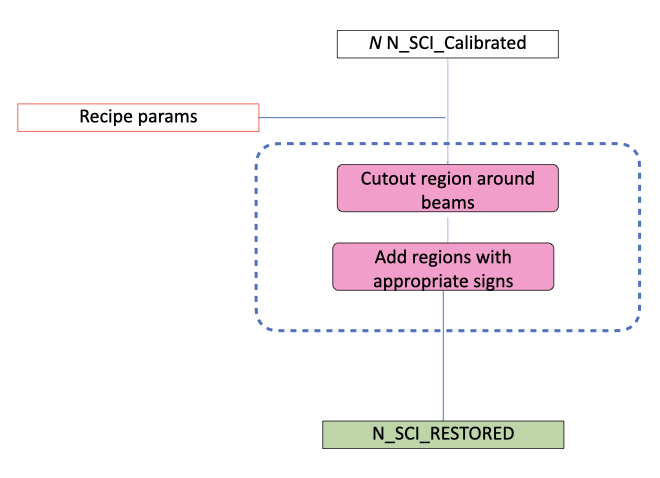
\includegraphics[width=0.9\textwidth]{metis_n_img_restore}
    \notgenerated{flowchart: hand-drawn; the recipe declares no steps}
  \caption[Recipe: \REC*{metis_n_img_restore}]{\REC*{metis_n_img_restore} --
    Create a single positive image from chop-nod difference image}
  \label{fig:metis_n_img_restore}
\end{figure}

%%%%%%%%%%%%%%
\clearpage
\subsubsection{\REC*{metis_n_img_distortion}:  Distortion calibration}
\label{rec:metis_n_img_distortion}
\label{n_img_distortion}
\label{rec:n_img_distortion}
\label{sssec:n_img_distortion}

Calibration of the imaging distortion is done on an image of a pin
hole mask located in a focal plane within the instrument. The
distortion is described in terms of a polynomial model whose
coefficients can be transformed to WCS keywords and applied to any
other pipeline product. In addition to the distortion table, a map of
pixel scale across the detector will be created.

\begin{recipedef}
  Name:                & \REC{metis_n_img_distortion} \\
  Purpose:             & Determine optical distortion coefficients for the N imager. \\
%  Requirements:        & \REQ{METIS-XXXX} \\
%  Type:                & Calibration | Science | Technical \\
%  Templates:           & \TPL{...} \\
  Primary input:       & \RAW{N_DISTORTION_RAW} (N$\times$) \\
                       & \RAW{N_WCU_OFF_RAW} (N$\times$) \\
  Secondary inputs:    & \PROD{BADPIX_MAP_GEO} (optional) \\
                       & \hyperref[dataitem:gain_map_det]{\STATCALIB*{GAIN_MAP_GEO}} \\
                       & \hyperref[dataitem:linearity_det]{\PROD*{LINEARITY_GEO}} \\
                       & \EXTCALIB{PERSISTENCE_MAP} (optional) \\
                       & \EXTCALIB{PINHOLE_TABLE} \\
  Matched keywords:    & \FITS{DRS.FILTER} \\
  Parameters:          & \CODE{metis_n_img_distortion.stacking.method}\newline Name of the method used to combine the input images (\texttt{add}, \texttt{average}, \texttt{median}, \texttt{sigclip}), default \texttt{average} \\
  Algorithm:           & Subtract background image with \texttt{hdrl\_imagelist\_sub\_image}. \\
                       & Measure location of point source images in frames with \texttt{hdrl\_catalogue\_create}. \\
                       & Call metis\_fit\_distortion to fit polynomial coefficients to deviations from grid positions. \\
  Output data:         & \PROD{N_DISTORTION_MAP} \\
                       & \PROD{N_DIST_REDUCED} \\
                       & \PROD{N_DISTORTION_TABLE} \\
%  Expected accuracies: & \\
  QC1 parameters:      & \QC{QC N DISTORT NSOURCE} \\
                       & \QC{QC N DISTORT RMS} \\
\end{recipedef}



\newgeometry{bottom=0.5cm, right=0.5cm, left=0.5cm}
\begin{figure}[hb]
    \centering
    \def \globalscale {0.700000}
    \fontsize{10}{12}\selectfont
    %% Flowchart of metis_n_img_distortion, generated by metisp/drld/generate_drld.py -- do not edit

% ADDING NEW DEFINITIONS -------------------------------------------- start
\definecolor{listingbg}{gray}{0.95}
\definecolor{darkgreen}{rgb}{0.0, 0.7, 0.0}
\definecolor{darkblue} {rgb}{0.0, 0.0, 0.7}
\definecolor{cyan} {rgb}{0.0, 0.4, 0.4}
\definecolor{darkred}  {rgb}{0.7, 0.0, 0.0}
\definecolor{darkorange}{rgb}{1.0, 0.49, 0.0}
\definecolor{violet}{rgb}{255, 0, 255}
\definecolor{turq}{rgb}{0.0, 0.7, 0.8}
\definecolor{fits}{rgb}{0.4, 0.1, 1}


\makeatletter
\lstdefinestyle{RAWstyle}{%
  basicstyle=\ttfamily\color{black}%
  \lst@ifdisplaystyle\scriptsize\fi}

\lstdefinestyle{PARstyle}{%
  basicstyle=\ttfamily\color{black}%
  \lst@ifdisplaystyle\scriptsize\fi}

\lstdefinestyle{DRLstyle}{%
  basicstyle=\ttfamily\color{black}%
  \lst@ifdisplaystyle\scriptsize\fi}

\lstdefinestyle{RECstyle}{%
  basicstyle=\ttfamily\color{black}%
  \lst@ifdisplaystyle\scriptsize\fi}

\lstdefinestyle{QCstyle}{%
  basicstyle=\ttfamily\color{black}%
  \lst@ifdisplaystyle\scriptsize\fi}

\lstdefinestyle{TPLstyle}{%
  basicstyle=\ttfamily\color{black}%
  \lst@ifdisplaystyle\scriptsize\fi}

\lstdefinestyle{PRODstyle}{%
  basicstyle=\ttfamily\color{black}%
  \lst@ifdisplaystyle\scriptsize\fi}

\lstdefinestyle{EXTCALIBstyle}{%
  basicstyle=\ttfamily\color{black}%
  \lst@ifdisplaystyle\scriptsize\fi}

\lstdefinestyle{STATCALIBstyle}{%
  basicstyle=\ttfamily\color{black}%
  \lst@ifdisplaystyle\scriptsize\fi}

\lstdefinestyle{FITSstyle}{%
  basicstyle=\ttfamily\color{black}%
  \lst@ifdisplaystyle\scriptsize\fi}
\makeatother

\input{recipe_config}
%% The picture is set in a box and only scaled down when it would not fit the page.
\ifdefined\flowchartbox\else\newsavebox{\flowchartbox}\fi
\sbox{\flowchartbox}{%
\begin{tikzpicture}
  [x=1cm,
  y=-1cm,
  align=center,
  node distance=2cm and 3.5cm,
  redstep/.append style={minimum height=0.8cm, text width=3.8cm}]
  \sffamily
  \pic (start){start};
  \node (input) [below=0.75cm of start-m, input] {%
    \textsl{N} \RAW{N_DISTORTION_RAW} \\[-0.5ex] {\footnotesize or} \\[-0.5ex]
    \textsl{N} \RAW{N_WCU_OFF_RAW}};

  %% algorithm steps
  \node (step_detectorsignatureremoval) [below=4.6cm of input, redstep]{%
    detector signature removal};
  \node (step_subtractwcuoffdark) [below=0.6cm of step_detectorsignatureremoval, redstep]{%
    subtract WCU OFF dark};
  \node (step_locateimages) [below=1.25cm of step_subtractwcuoffdark, redstep]{%
    locate images};
  \node (step_fitpolynomial) [below=0.6cm of step_locateimages, redstep]{%
    fit polynomial};
  \pic (stop) [below=3.45cm of step_fitpolynomial] {stop};

  \draw [connection_arrow] (start-m) -- (input);
  \draw [connection_arrow] (input) -- (step_detectorsignatureremoval);
  \draw [connection_arrow] (step_detectorsignatureremoval) -- (step_subtractwcuoffdark);
  \draw [connection_arrow] (step_subtractwcuoffdark) -- (step_locateimages);
  \draw [connection_arrow] (step_locateimages) -- (step_fitpolynomial);
  \draw [connection_arrow] (step_fitpolynomial) -- (stop-t);

  %% calibration inputs, attached above the step that consumes them
  \node (connect_badpixmap) [connection] at ($(input.south) + (0, 0.97)$) {};
  \node (badpixmap) [left=of connect_badpixmap, calproduct] {\PROD{BADPIX_MAP_GEO}};
  \draw [connection_arrow, dashed] (badpixmap) -- (connect_badpixmap);
  \node (connect_gainmap) [connection] at ($(input.south) + (0, 1.98)$) {};
  \node (gainmap) [left=of connect_gainmap, external] {\hyperref[dataitem:gain_map_det]{\STATCALIB*{GAIN_MAP_GEO}}};
  \draw [connection_arrow] (gainmap) -- (connect_gainmap);
  \node (connect_linearity) [connection] at ($(input.south) + (0, 2.98)$) {};
  \node (linearity) [left=of connect_linearity, calproduct] {\hyperref[dataitem:linearity_det]{\PROD*{LINEARITY_GEO}}};
  \draw [connection_arrow] (linearity) -- (connect_linearity);
  \node (connect_persistencemap) [connection] at ($(input.south) + (0, 3.98)$) {};
  \node (persistencemap) [left=of connect_persistencemap, external] {\EXTCALIB{PERSISTENCE_MAP}};
  \draw [connection_arrow, dashed] (persistencemap) -- (connect_persistencemap);
  \node (connect_pinholetable) [connection] at ($(step_subtractwcuoffdark.south) + (0, 0.62)$) {};
  \node (pinholetable) [left=of connect_pinholetable, external] {\EXTCALIB{PINHOLE_TABLE}};
  \draw [connection_arrow] (pinholetable) -- (connect_pinholetable);

  %% products, attached below the step that produces them
  \node (connect_distortionmap) [connection] at ($(step_fitpolynomial.south) + (0, 0.62)$) {};
  \node (distortionmap) [right=of connect_distortionmap, calproduct] {\PROD{N_DISTORTION_MAP}};
  \draw [connection_arrow] (connect_distortionmap) -- (distortionmap);
  \node (connect_distortionreduced) [connection] at ($(step_fitpolynomial.south) + (0, 1.62)$) {};
  \node (distortionreduced) [right=of connect_distortionreduced, calproduct] {\PROD{N_DIST_REDUCED}};
  \draw [connection_arrow] (connect_distortionreduced) -- (distortionreduced);
  \node (connect_distortiontable) [connection] at ($(step_fitpolynomial.south) + (0, 2.62)$) {};
  \node (distortiontable) [right=of connect_distortiontable, calproduct] {\PROD{N_DISTORTION_TABLE}};
  \draw [connection_arrow] (connect_distortiontable) -- (distortiontable);

  \draw [frame] ($(input.south) + (-2.85, 0.12)$) rectangle
  ($(step_fitpolynomial.south) + (2.85, 3.0500000000000003)$);
  \node [framecolor, anchor=north west] at ($(input.south) + (-2.85, 0.12)$) {%
    \REC{metis_n_img_distortion}};
\end{tikzpicture}}%
\ifdim\ht\flowchartbox>\dimexpr\textheight-4\baselineskip\relax
  \resizebox{!}{\dimexpr\textheight-4\baselineskip\relax}{\usebox{\flowchartbox}}%
\else\ifdim\wd\flowchartbox>\linewidth
  \resizebox{\linewidth}{!}{\usebox{\flowchartbox}}%
\else
  \usebox{\flowchartbox}%
\fi\fi

% ADDING NEW DEFINITIONS -------------------------------------------- start
\definecolor{listingbg}{gray}{0.95}
\definecolor{darkgreen}{rgb}{0.0, 0.7, 0.0}
\definecolor{darkblue} {rgb}{0.0, 0.0, 0.7}
\definecolor{cyan} {rgb}{0.0, 0.4, 0.4}
\definecolor{darkred}  {rgb}{0.7, 0.0, 0.0}
\definecolor{darkorange}{rgb}{1.0, 0.49, 0.0}
\definecolor{violet}{rgb}{255, 0, 255}
\definecolor{turq}{rgb}{0.0, 0.7, 0.8}
\definecolor{fits}{rgb}{0.4, 0.1, 1}


\makeatletter
\lstdefinestyle{RAWstyle}{%
  basicstyle=\ttfamily\color{fits}%
  \lst@ifdisplaystyle\scriptsize\fi}

\lstdefinestyle{PARstyle}{%
  basicstyle=\ttfamily\color{cyan}%
  \lst@ifdisplaystyle\scriptsize\fi}

\lstdefinestyle{DRLstyle}{%
  basicstyle=\ttfamily\color{violet}%
  \lst@ifdisplaystyle\scriptsize\fi}

\lstdefinestyle{RECstyle}{%
  basicstyle=\ttfamily\color{darkgreen}%
  \lst@ifdisplaystyle\scriptsize\fi}

%% Write QC parameters like this: \QC{QC_SOMETHING_OR_OTHER}
\lstdefinestyle{QCstyle}{%
  basicstyle=\ttfamily\color{darkblue}%
  \lst@ifdisplaystyle\scriptsize\fi}

%% Write templates like this: \TPL{DARK_LM}
\lstdefinestyle{TPLstyle}{%
  basicstyle=\ttfamily\color{darkred}%
  \lst@ifdisplaystyle\scriptsize\fi}

%% Write products like this: \PROD{SOME_THING}
\lstdefinestyle{PRODstyle}{%
  basicstyle=\ttfamily\color{darkorange}%
  \lst@ifdisplaystyle\scriptsize\fi}

%% external calib files
\lstdefinestyle{EXTCALIBstyle}{%
  basicstyle=\ttfamily\color{Turquoise}%
  \lst@ifdisplaystyle\scriptsize\fi}

% static calib files
\lstdefinestyle{STATCALIBstyle}{%
  basicstyle=\ttfamily\color{teal}%
  \lst@ifdisplaystyle\scriptsize\fi}

% static calib files
\lstdefinestyle{FITSstyle}{%
  basicstyle=\ttfamily\color{black}%
  \lst@ifdisplaystyle\scriptsize\fi}
\makeatother


  \caption[Recipe: \REC*{metis_n_img_distortion}]{%
    \REC{metis_n_img_distortion} -- \CODE{IMG_N} distortion calibration}
  \label{fig:metis_n_img_distortion}
\end{figure}
\restoregeometry

%%% Local Variables:
%%% TeX-master: "METIS_DRLD"
%%% End:
